\documentclass[border=10pt, tikz]{standalone}
 \usepackage{tikz}
\usetikzlibrary{calc,shapes.geometric,shapes.symbols}

% http://tex.stackexchange.com/questions/303295/tikz-and-pgfdeclareshape-why-the-text-is-not-at-the-center-anchor/303298#303298


\tikzset{%
couleur/.style={fill={#1},top couleur/.style={fill=#1!50}},%
}%

\makeatletter%

\pgfkeys{/tikz/remplissage/.initial = -1
  cm}%hauteur de fluide -1 = vide




% ---------------- %
% erlenmeyer %
% ---------------- %
\pgfdeclareshape{erlenmeyer}{%
  \nodeparts{text}%
  \savedanchor{\lowerlefttextcorner}{
    \pgf@y=-0.5\ht\pgfnodeparttextbox % height of the box, ignoring the depth
    \pgf@x=-0.5\wd\pgfnodeparttextbox % width of the box
  }%



  \anchor{center}{\pgfpoint{0}{0cm}}%
  \anchor{north}{\pgfpoint{0}{1.85cm}}%
  \anchor{south}{\pgfpoint{0}{-2cm}}%

  \anchor{text}{%
    \lowerlefttextcorner%
  }%

  \saveddimen\hauteurphase{\pgf@x=\pgfkeysvalueof{/tikz/remplissage}}%

  \behindbackgroundpath{ %
    \path[draw,clip] (-0.5,1.75) to[rounded
    corners=2pt]++(0,-1)to[rounded corners=10pt]++(-1,-2.5)to[rounded
    corners=10pt, bend right=15pt]++(3,0) to[rounded
    corners=2pt]++(-1,2.5)--++(0,1)++(-0.5,0) circle [x radius=0.5, y
    radius=0.1];%
    \path[couleur](-1.6,-2) rectangle (1.6,{\hauteurphase-2cm});
    \path[draw=white,top couleur] (0,\hauteurphase-2cm) circle [x
    radius=1.5cm-(\hauteurphase-0.25cm)*0.4 , y
    radius=0.1 cm];%
  }%
}





\makeatother

\begin{document}

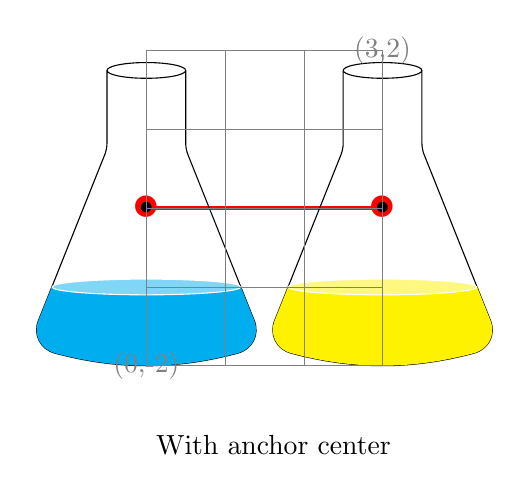
\begin{tikzpicture}[anchor=center, remplissage = 1cm]
  \draw[red, ultra thick] (0,0)node[scale=2]{$\bullet$} --(3,0) node[scale=2]{$\bullet$};%

  \draw (0,0)node[erlenmeyer, couleur = cyan]{$\bullet$}
  ++ (3,0)node[erlenmeyer, couleur = yellow]{$\bullet$};%

  \draw [help lines] (0,-2) node{(0,-2)}grid(3,2)node{(3,2)};%

\draw (0,-3)node[right]{With anchor center};
\end{tikzpicture}

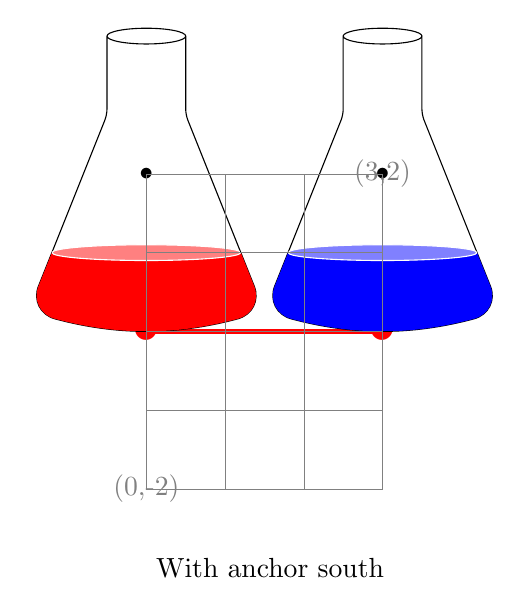
\begin{tikzpicture}[ remplissage = 1cm]
  \draw[red, ultra thick] (0,0)node[scale=2]{$\bullet$} --(3,0) node[scale=2]{$\bullet$};%

  \draw (0,0)node[erlenmeyer,anchor=south, couleur = red]{$\bullet$}
  ++ (3,0)node[erlenmeyer ,above, couleur = blue]{$\bullet$};%

  \draw [help lines] (0,-2) node{(0,-2)}grid(3,2)node{(3,2)};%

\draw (0,-3)node[right]{With anchor south};

\end{tikzpicture}

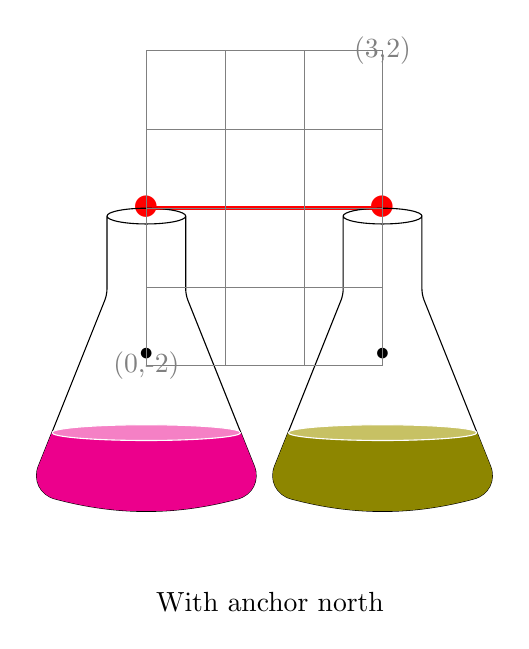
\begin{tikzpicture}[remplissage = 1cm]
  \draw[red, ultra thick] (0,0)node[scale=2]{$\bullet$} --(3,0)
  node[scale=2]{$\bullet$};%

  \draw (0,0)node[erlenmeyer, anchor=north, couleur = magenta]{$\bullet$}
  ++ (3,0)node[erlenmeyer, anchor=north, couleur = olive]{$\bullet$};%

 \draw [help lines] (0,-2) node{(0,-2)}grid(3,2)node{(3,2)};%
\draw (0,-5)node[right]{With anchor north};

\end{tikzpicture}

\end{document}